\documentclass[tikz,border=4pt]{standalone}
\usepackage[T1]{fontenc}
\usepackage{lmodern}
\renewcommand{\familydefault}{\sfdefault}
\usetikzlibrary{shapes.geometric,positioning,arrows.meta,calc,fit,backgrounds,decorations.pathreplacing}
\tikzset{
  node distance=6mm,
  every node/.style={font=\footnotesize,align=center,execute at begin node={\hyphenpenalty=10000\relax}},
  base/.style={draw=gray!60,fill=gray!12,minimum height=7mm,inner sep=2pt},
  term/.style={base,rounded corners=3.5mm,text width=30mm},
  proc/.style={base,text width=32mm},
  err/.style={base,text width=30mm,fill=gray!22},
  io/.style={base,trapezium,trapezium left angle=72,trapezium right angle=108,trapezium stretches=true,text width=28mm},
  dec/.style={base,diamond,aspect=2.4,text width=27mm,inner sep=0pt},
  % predefined process: a call to another procedure
  sub/.style={proc,inner xsep=3mm,path picture={
    \draw[gray!60] ([xshift=1.5mm]path picture bounding box.north west)--([xshift=1.5mm]path picture bounding box.south west)
                   ([xshift=-1.5mm]path picture bounding box.north east)--([xshift=-1.5mm]path picture bounding box.south east);}},
  go/.style={-{Stealth[length=2mm]},draw=gray!55!black},
  lab/.style={font=\scriptsize,fill=white,inner sep=1pt},
  frame/.style={draw=gray!60,dashed,rounded corners=2mm,inner sep=3mm},
  % memory diagrams
  cell/.style={draw=gray!60,fill=gray!12,minimum height=7mm,inner sep=1pt,font=\scriptsize},
  hot/.style={cell,fill=gray!35},
  note/.style={font=\scriptsize,text=gray!30!black},
}

\begin{document}
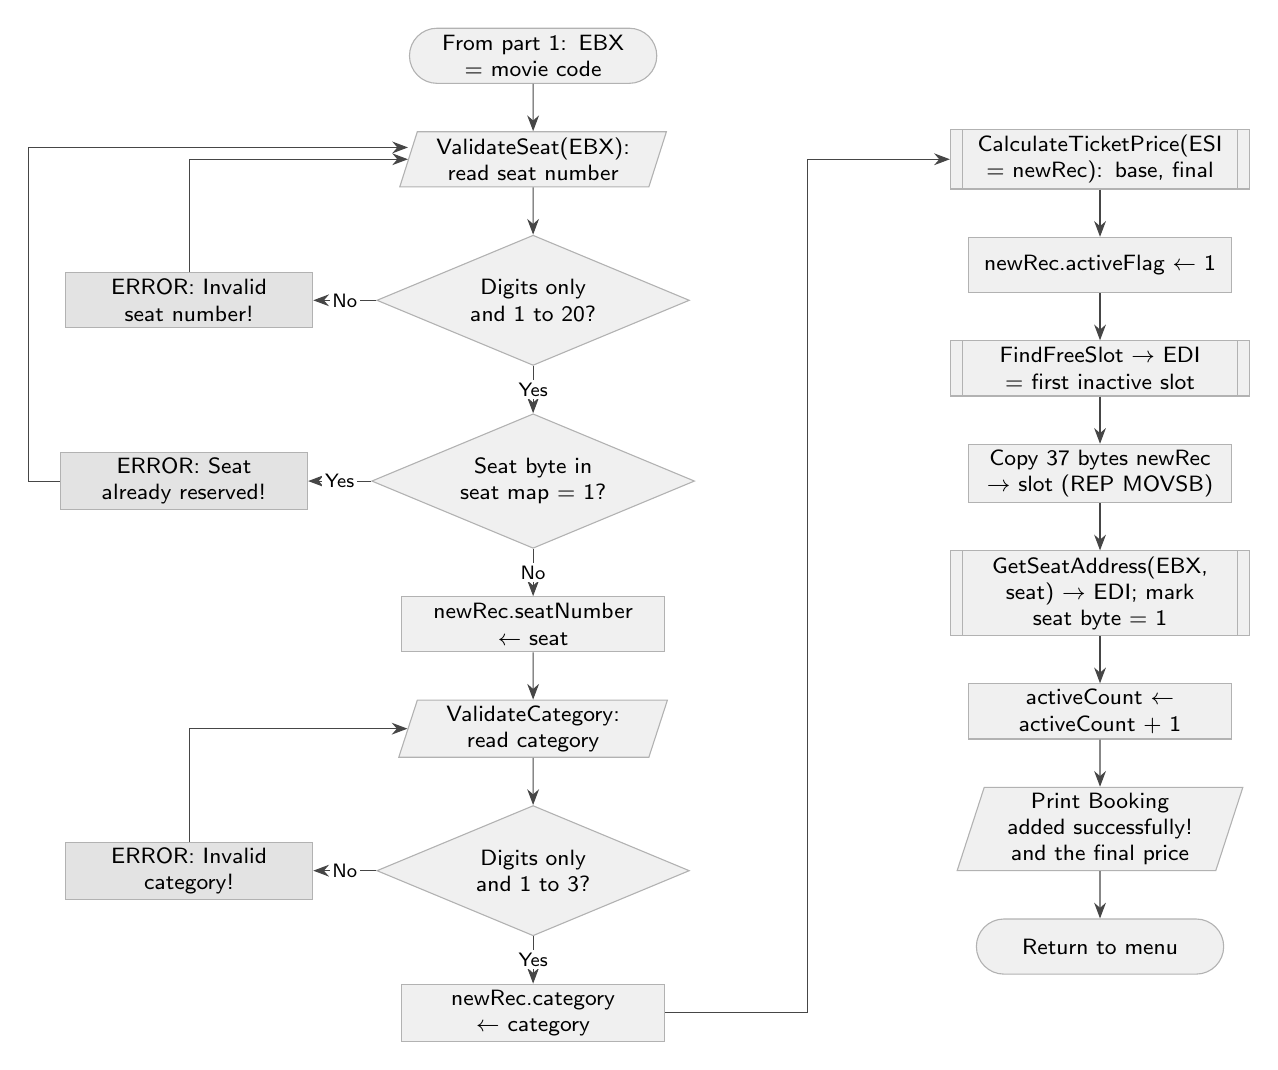
\begin{tikzpicture}
\node[term] (s) {From part 1: EBX = movie code};
\node[io,below=of s] (rs) {ValidateSeat(EBX): read seat number};
\node[dec,below=of rs] (d1) {Digits only and 1 to 20?};
\node[err,left=8mm of d1] (e1) {ERROR: Invalid seat number!};
\node[dec,below=of d1] (d2) {Seat byte in seat map = 1?};
\node[err,left=8mm of d2] (e2) {ERROR: Seat already reserved!};
\node[proc,below=of d2] (ss) {newRec.seatNumber $\leftarrow$ seat};
\node[io,below=of ss] (rc) {ValidateCategory: read category};
\node[dec,below=of rc] (d3) {Digits only and 1 to 3?};
\node[err,left=8mm of d3] (e3) {ERROR: Invalid category!};
\node[proc,below=of d3] (sc) {newRec.category $\leftarrow$ category};
\node[sub] (pr) at ($(rs)+(72mm,0)$) {CalculateTicketPrice(ESI = newRec): base, final};
\node[proc,below=of pr] (fl) {newRec.activeFlag $\leftarrow$ 1};
\node[sub,below=of fl] (ff) {FindFreeSlot $\rightarrow$ EDI = first inactive slot};
\node[proc,below=of ff] (cp) {Copy 37 bytes newRec $\rightarrow$ slot (REP MOVSB)};
\node[sub,below=of cp] (gs) {GetSeatAddress(EBX, seat) $\rightarrow$ EDI; mark seat byte = 1};
\node[proc,below=of gs] (ac) {activeCount $\leftarrow$ activeCount + 1};
\node[io,below=of ac] (ok) {Print Booking added successfully! and the final price};
\node[term,below=of ok] (r) {Return to menu};
\draw[go] (s)--(rs);
\draw[go] (rs)--(d1);
\draw[go] (d1)--node[lab]{No}(e1);
\draw[go] (e1.north)|-(rs.west);
\draw[go] (d1)--node[lab]{Yes}(d2);
\draw[go] (d2)--node[lab]{Yes}(e2);
\draw[go] (e2.west)--++(-4mm,0)|-([yshift=1.5mm]rs.west);
\draw[go] (d2)--node[lab]{No}(ss);
\draw[go] (ss)--(rc);
\draw[go] (rc)--(d3);
\draw[go] (d3)--node[lab]{No}(e3);
\draw[go] (e3.north)|-(rc.west);
\draw[go] (d3)--node[lab]{Yes}(sc);
\draw[go] (sc.east)-|($(sc.east)!0.5!(sc.east -| pr.west)$)|-(pr.west);
\foreach \a/\b in {pr/fl,fl/ff,ff/cp,cp/gs,gs/ac,ac/ok,ok/r}{\draw[go] (\a)--(\b);}
\end{tikzpicture}
\end{document}
